\section{Some theoretical background: } 

GIFMOD is equipped with two inverse modeling modules including a maximum-likelihood (deterministic) parameter estimation and a Bayesian probabilistic parameter estimation. The deterministic parameter estimation approach uses a Hybrid Genetic Algorithm to find combination of model parameters maximizing the likelihood of observing the measured data which the Bayesian approach uses Markov Chain Monte Carlo (MCMC) algorithm to produce samples of parameters representing the joint posterior distribution of model parameters designated to be estimated by the program. 

GIFMOD allows for any of the parameters in the model to be treated as unknown parameters and be estimated by providing their prior distributions while allowing the user to choose between three types of prior distributions: including normal, log-normal, and uniform. 
The observed data can be specified to represent any of the state variables in the model including hydraulic (i.e.  flow rates, head, cross- sectional areas), as well as particle and constituent concentrations at each block. As is typically done in Bayesian inference, the error here is defined as a quantity encompassing measurement error, model structural error, and all other errors resulting from the uncertainties associated with the external forcing (input data) such as weather data, inflow rates, and concentrations, etc. The general form of the model error structure can be expressed using the following equation: 

\begin{equation}
\label{eq:im1}
\tilde Y(t) = \xi^{-1}[\xi[Y(t)]+\epsilon]
\end{equation}
where $Y$ is the vector containing the model’s observed constituents, $\tilde Y(t)$ represents the observed data vector, $\xi$ represents the error structure function (e.g., for log-normal error structure, $\xi$ is the natural logarithm function, while for Gaussian error structure, $\xi$ is the identity function), and $\epsilon$ is a random vector containing transformed measurement, structural and external forcing errors, which is assumed to collectively follow a multivariate normal distribution. 
The Bayes’ theorem \citep{kaipio2006} can be used to obtain the joint probability distribution of parameters given the observed data, namely, the posterior distribution of the parameters as:
\begin{equation}
\label{eq:im2}
p(\vec{\Psi}|\vec{\tilde Y})=\frac{p(\vec{\tilde Y}|\vec{\Psi}) p(\vec{\Psi})}{p(\vec{\tilde Y})}
\end{equation}

where $p(\vec{\tilde Y}|\Psi)$ is the likelihood function that is the probability of observing the measured data $\vec{\tilde Y}$ given a parameter set $\vec{\Psi}$, $p(\vec{\Psi})$ represents the prior knowledge about the parameters and error structure, and $p(\vec{\tilde Y})$ is a normalizing factor. $\vec{\Psi}$ in Eq. (\ref{eq:im2}) contains all the parameters that are intended to be estimated using the observed data and the elements of the variance-covariance matrix for the random error term $\epsilon$ in eq. (\ref{eq:im1}). The likelihood of observing $\vec{\tilde Y}(t)$ given a parameter set $\vec{\Psi}$ or simply the likelihood function $p(\vec{\tilde Y}|\Psi) = p(\vec{\tilde Y}|\vec{Y},\vec{\Gamma})$ can be theoretically calculated based on the error structure. If the errors due to the uncertainties associated with the external forcing are considered part of the observation error, then the external forcing can be considered deterministically, and thus the model outputs become a function of only model parameters. In this case, the error function can be re-written as $p(\vec{\tilde Y}|\vec{\Phi},\vec{\Gamma})$. In theory, each element of the variance-covariance matrix $\vec{\Gamma}$ should be estimated as part of the parameter estimation. However, this makes the total number of parameters to be estimated very large and imposes a large computational burden. Therefore, observation errors of different constituents are typically assumed to be independent, and the correlations between observed concentration errors of different constituents are ignored \citep{walsh2012}. By making this assumption, the variance-covariance matrix becomes diagonal. If it is also assumed that errors of consecutive observations of individual data-sets used in parameter estimation are independent of each other, then the likelihood function of the observed vector can be computed as a function of the model parameters:
\begin{equation}
\label{eq:im3}
p(\vec{\tilde Y}|\vec{\Psi})=\frac{\prod_{i=1}^{NT} \prod_{j=1}^{NS_i} \xi'(\tilde y_{ij})}{(2 \pi \prod_{i=1}^{NT} \sigma_i^2)^{NS_i/2}}exp\bigg[-\sum_{i=1}^{NT} \sum_{j=1}^{NS_i} \frac{(y_{ij}-\tilde y_{ij})^2}{2 \sigma_i^2}\bigg]
\end{equation}

where $\tilde y_{ij}\in \vec{\tilde Y}$ is the $j^{th}$ data point of observed concentration of observed state variable $i$, $NT$ is the total number of different measured state variables, $j$ indicates the time and location of the measurement. $NS_i$ is the number of total samples (in time or location) of observed state variable $i$. The mapping function $\xi$ in the likelihood function can be assumed to be any transformation depending on the distribution of the observed data or by performing trial and error to find the best transformation by comparing the posterior residuals with the presumed error structure, and $\xi'$ is its derivative. For example, considering $\xi$ to be the identity function implies a normally distributed and additive error structure, while assuming $\xi$ to be the logarithm function results in a log-normally distributed and multiplicative error structure. Other error structures can be obtained by selecting a corresponding mapping function. $y_{ij}\in \vec{Y}$  is the predicted concentration of constituent $i$ at time/location $j$. $\sigma_i$ is the standard deviation of observed constituent $i$. When the deterministic parameter estimation approach based on maximum likelihood approach is to be applied to estimate the parameters, the values of parameters that maximize Eq. \ref{eq:im3} \citep{montgomery2010} are found  using a hybrid genetic algorithm. 
The second term in the numerator of Eq. \ref{eq:im2} represents the prior knowledge about the probability density of the parameters. This information can be obtained from literature reviews, experts’ experience, or independently performed experimental results.
In the probabilistic parameter estimation module, the MCMC algorithm \citep{gamerman2006} is used to generate random samples according to the posterior distribution in Eq. \ref{eq:im2}. The MCMC algorithm implemented in the program is based on the Metropolis-Hasting method \citep{metropolis1953}. MCMC algorithm that is implemented into GIFMOD automatically adjusts the perturbation factors to achieve an acceptance rate provided by the user. In the next section the way to set up an inverse problem in GIFMOD and the parameters adjusted by the user in order to do so are described.  
\section{Defining parameters and observed data}
In order to perform an inverse modeling, parameters and observed data should first be introduced. Parameters should be assigned to the specific properties of the model and each set of observed data should be attributed to a specific output of the model. 
\subsection{Defining parameters and adjusting their properties: }
In order to add a parameter to the model right click on \textbf{Inverse Modeling}$\rightarrow$\textbf{Parameters} and then click on \textbf{Add parameters}. Each parameter has the following properties: 

\begin{itemize}
    \item \textbf{Name: } This indicates the name that is assigned to a parameter. The name of the parameter will be used to assign the parameter to specific properties of the model and when generating the results of inverse modeling.
    \item \textbf{Value: } This is the value that will be assigned to the parameter if the modeling is conducted in forward mode. 
    \item \textbf{Maximum Value: } In deterministic inverse modeling, this indicates the upper bound for the parameter (search domain). In probabilistic inverse modeling, it indicates the 97.5 percentile of the prior distribution for this parameter. 
    \item \textbf{Minimum Value: } In deterministic inverse modeling, this indicates the lower bound for the parameter (search domain). In probabilistic inverse modeling, it indicates the 2.5 percentile of the prior distribution for this parameter.
    \item \textbf{Prior distribution: } Indicates the mathematical form of the prior distribution of the parameters. The choices provided include \textbf{Normal}, and \textbf{Lognormal}. The mean and standard deviation of the prior distributions are calculated based on the maximum and minimum values. 
\end{itemize}

\subsection{Defining observed data and assigning their properties: }
Observed data can be added by right-clicking on \textbf{Inverse Modeling}$\rightarrow$\textbf{Observations} and then clicking on \textbf{Add observation}. Each observation includes a time-series representing an state variable of the model. Each observation has the following properties: 

\begin{itemize}
    \item \textbf{Name: } The name of an observation is used when generating results in deterministic and probabilistic inverse modeling. 
    \item \textbf{Standard Deviation ID: } This is an identification that is used to group observations that will be assigned the same standard deviation. The total number of groups of observations is equivalent to the parameter $NT$ in Eq. \ref{eq:im3}. The observations having the same \textbf{Standard Deviation ID} will be grouped together and a single observation error standard deviation, $\sigma_i$ will be assigned to them. 
    \item \textbf{Block/connector: } This indicates whether the state variable to the observation correspond to is a block or a connector state variable. Concentrations, storages, hydraulic heads are always block state variables, while flow rates and interface areas are connector state variables. 
    \item \textbf{Error distribution: } This indicates the error structure ($\xi$) in Eq. \ref{eq:im1} that is used when computing the likelihood value.
    \item \textbf{Location: } Indicate the block or the connector that this observed data corresponds to. 
    \item \textbf{Observed data: } This field allows loading the observed data time-series. The observed data time series is a .csv text file that should consist of two columns first representing times of measurement and the second the observed values. 
    \item \textbf{Quantity: } This field allows selecting the state variable that the observed data corresponds to. As for water quality and particles the drop-down menu containing the selectable state variables is populated depending on the constituents, phases, and particle types available. 
    
\end{itemize}
\subsection{Example: Estimation of bio-kinetic parameters of nitrification processes from an batch test: }
This case represent interpretation of an actual experiment to determine the rates of microbial activities during ammonia and nitrite oxidation. Four experiments were conducted using the same sludge sample. The variation of dissolved oxygen with respect to time was measured for each of the four experiments. The initial conditions for each of the experiments is shown in Table \ref{table:inverse_example} and the observed variation of DO for the four cases are shown in Figure \ref{fig:inverse_example1}. 

\begin{table}[]
    \centering
    \begin{tabular}{c|c c c c}
       Experiment  & $NO_3^{-1}(mg/L) $ & $NH_3(mg/L)$ & $DO(mg/L)$ & $VSS(mg/L)$ \\
    \hline
        No Spike & 0 & 0 & UK* &  730  \\
        $NO_2^{-1}$ Spike & 50 & 0 & UK & 695 \\
        $NH_3$ Spike & 0 & 50 & UK & 645 \\
        $NO_2^{-1}$ and $NH_3$ & 50 & 50 & UK & 660\\ 
    \end{tabular}
    \caption{Initial condition for the declining DO test aimed at estimating AOB and NOB biokinetics. *- UK: The initial condition for DO is treated as a parameter to be estimated by the model}
    \label{table:inverse_example}
\end{table}

The processes considered in the model are shown in table \ref{table:inverse_example2}. The only constituents that will be explicitly considered in the model include $DO$, $NH_3$, $NO_2^{-1}$, and $VSS$. $VSS$ is used as a surrogate for biomass (i.e. it is assumed to be proportional to AOB, NOB and OHO) and it is also assumed to stay unchanged throughout each experiment. the Petersen matrix is shown in table \ref{table:inverse_example3}.

\begin{figure}[!ht]
\begin{center}
\includegraphics[width=6cm]{Images/Figure35.png} \\
\caption{Temporal variation of DO for the four different experiments used to estimate nitrification bio-kinetics parameters}\label{fig:inverse_example1}
\end{center}
\end{figure}

\begin{table}[]
    \centering
    \begin{tabular}{l l}
       Process & Reaction Expression \\
    \hline
        Ammonia oxidation (AO) & $21.9O_2 + \frac{21.9}{3.43}NH_3 \rightarrow \frac{21.9}{3.43}NO_2^{-1}$  \\
        Nitrite oxidation (NO) & $11.7O_2 + \frac{11.7}{1.14}NO_2^{-1} \rightarrow \frac{11.7}{1.14}NO_3^{-1}$ \\
        Ordinary heterotrophic growth (OHO) & $BOD + O_2 \rightarrow CO_2$ \\
    \end{tabular}
    \caption{Reactions considered in the nitrification bio-kinetics parameter estimation example}
    \label{table:inverse_example2}
\end{table}


\begin{table}[]
    \centering
    \begin{tabular}{l|c |c c c c}
       Process & Rate Expression & $O_2$ & $NH_3$ & $NO_2^{-1}$ & VSS  \\
    \hline
        AO & $VSS \mu_{AOB} \frac{[O_2]}{(k_{OA} + [O_2]}\frac{[NH_3]}{[NH_3]+k_{NH3}}$ & -21.9 & $-\frac{21.9}{3.43}$ & $\frac{21.9}{3.43}$ &   \\
        NO & $VSS \mu_{NOB} \frac{[O_2]}{k_{ON} + [O_2]}\frac{[NO_2^{-1}]}{[NO_2^{-1}]+k_{NO2}}$ & $-11.7$ &  & $-\frac{11.7}{1.14}$ &   \\
        OHO & $VSS \mu_{OHO} \frac{[O_2]}{k_{OH}+[O_2]}$ & $-\frac{1-0.52}{0.52}$ & & &  \\
    \end{tabular}
    \caption{Petersen matrix for the nitrification bio-kinetics parameter estimation example}
    \label{table:inverse_example3}
\end{table}

\begin{table}[]
    \centering
    \begin{tabular}{l|c c c}
       Parameter & 2.5\% & 97.5\% & Distribution  \\
    \hline
        $\mu_{AOB}$ & 0.005 & 0.5 & lognormal \\
        $k_{OA}$ & 0.05 & 2.0 & lognormal \\
        $\mu_{NOB}$ & 0.005 & 0.5 & lognormal \\
        $k_{ON}$ & 0.05 & 2.0 & lognormal \\
        $k_{NH3}$ & & FIXED = 0.5 & \\
        $k_{NO2}$ & & FIXED = 0.5 & \\
        $\mu_{OHO}$ & 0.0001 & 0.1 & lognormal \\
        $k_{OH}$ & 0.00125 & 10 & lognormal \\
    \end{tabular}
    \caption{Prior range of parameters used in nitrification bio-kinetics example}
    \label{table:inverse_example4}
\end{table}

\begin{figure}[!ht]
\begin{center}
\includegraphics[width=12cm]{Images/Figure36.png} \\
\caption{Reaction network for the nitrification parameter estimation example}\label{fig:inverse_example2}
\end{center}
\end{figure}    


Table \ref{table:inverse_example4} shows the prior 95\% ranges and the prior distributions of each of the parameters. In this particular case due to lack of information about $NH_3$ and $NO_2^{-1}$ concentration variation with time if $k_{NH3}$, and $k_{NO2}$ are considered unknown, there is a risk of problem becoming over-parametrized and therefore, we here assume the values of these two parameters to be fixed.   

\subsubsection{Steps to set-up the model: }
To construct the model in GIFMod follow the following steps: 
\begin{itemize}
    \item \textbf{Add a pond: } We will simulate the reactor using a \textbf{Pond} block. Other media types can also be used. Add a pond by clicking on the pond icon 
\includegraphics[width=0.5cm]{Icons/pond_icon.png} on the top tool bar. Set the following properties for the pond: \\
    - \textbf{Area: } 1$m^2$\\
    - \textbf{Initial water depth: } 1m\\
    \item \textbf{Add the constituents: } Add constituents ($DO$, $NH_3$, $NO_2^{-1}$, $VSS$) by right-clicking on \textbf{Water quality}$\rightarrow$\textbf{Constituents}. \item \textbf{Adding experiments: } The goal of this example is to infer the values of reaction parameters using four experiments in a holistic way. This means that the best parameter set that can collectively explain the results from the four experiments in sought for. There are two ways to consider four experiments in the model. The first way is to define four independent ponds with different initial conditions and the second way is to use \textbf{Experiments}. Here we will use the second approach. \\ To add experiments click on the \textbf{Add new experiment} button 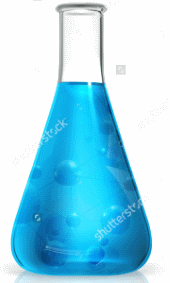
\includegraphics[width=0.3cm]{Icons/newexperiment_icon.png} three times to add three new experiments. 
    
    \item \textbf{Setting the duration of the simulation: } The duration of the experiments are all below 0.2 days. First from the experiment menu on the top tool bar select \textbf{All experiments}. This forces the program to apply any changes in the properties to all the experiments. To set the simulation duration to 0.2 from \textbf{Settings}$\rightarrow$\textbf{Project settings} and from the \textbf{Properties} window right-click on the label for \textbf{Simulation end time} and click on \textbf{Enter number} from the drop-down menu that appears. Enter 0.2 in the dialog box that appears. 
    
    \item \textbf{Adding reaction parameters: } Add the eight reaction parameters by right-clicking on \textbf{Water quality}$\rightarrow$\textbf{Reactions}$\rightarrow$\textbf{Reaction parameters} according to table \ref{table:inverse_example4}. For the two fixed parameters $k_{NH3}$ and $k_{NO2}$, enter a value of 0.5. 
    \textbf{Add reaction network: } Right click on reaction  \textbf{Water quality}$\rightarrow$\textbf{Reactions}$\rightarrow$\textbf{Reaction network}. Enter the processes according to the Petersen matrix shown in table \ref{table:inverse_example3}. The finished reaction network window should look like figure \ref{fig:inverse_example2}.\\
    \item \textbf{Setting initial conditions: } From the \textbf{Experiments} drop-down menu on the top tool bar, select \textbf{Experiment1}. Click on the pond block and then from the \textbf{Properties} window choose \textbf{Constituent initial conditions}. Enter the initial conditions for experiment 1 according to Table \ref{tab:inv_ini_cond}.
   \begin{table}[]
    \centering
    \begin{tabular}{l|c c c c}
       Experiment & $DO(mg/L)$ & $NH_3(mg/L)$ & $NO_2^{-1}(mg/L)$ & VSS (mg/L) \\
    \hline
        1 & 7.78 & 0 & 0 & 730 \\
        2 & 7.76 & 50 & 0 & 645 \\
        3 & 8.02 & 0 & 50 & 695 \\
        4 & 7.8 & 50 & 50 & 660 \\
    \end{tabular}
    \caption{Initial conditions for the four experiments used for estimation of bio-kinetics and stoichiometric parameters of nitrification}
    \label{tab:inv_ini_cond}
\end{table} 
    
    The initial condition window for the first experiment should look like Figure \ref{fig:42}. 
    
\begin{figure}[!ht]
\begin{center}
\includegraphics[width=6cm]{Images/Figure42.png} \\
\caption{Initial conditions for the nitrification inverse modeling example}\label{fig:42}
\end{center}
\end{figure}  

Change the experiment to experiment2 from the \textbf{experiments} drop down menu and similarly set the initial condition according to the second row of table \ref{tab:inv_ini_cond}. 

Similarly assign the initial conditions for experiment 3 and 4. 
    
    \item \textbf{Setting up parameters to be estimated: } Add a parameter representing $\mu_{AOB}$ by right-clicking of \textbf{Inverse modeling}$\rightarrow$\textbf{Parameters} and clicking on \textbf{Add parameters} from the drop-down menu. Assign the following parameter to the newly added parameter:\\
    - \textbf{Name:} $\mu_{AOB}$\\
    - \textbf{Maximum value: } \textit{0.5}\\
    - \textbf{Minimum value: } \textit{0.005}\\
    - \textbf{Distribution: } \textit{Log-Normal}\\
    Repeat for the other parameters to be estimated including $k_{OA}$, $\mu_{NOB}$, $k_{ON}$, $\mu_{OHO}$,
and $k_{OH}$ and assign the ranges and the distribution according to table \ref{table:inverse_example4}. As for the \textbf{Value} of the parameters respectively use $\mu_{AOB}=0.05$, $k_{OA}=0.31$, $\mu_{NOB}=0.05$, $k_{ON}=0.31$, $\mu_{OHO}=0.003162$, $k_{OH}=0.111$. These values are used when the model is run in forward mode. \\Please note that the name of the parameters should not be identical to their corresponding reaction parameters. \\


\item \textbf{Assigning the parameters to the corresponding model properties: } The parameters defined in the previous step should not be assigned to their corresponding properties in the model. Choose the reaction parameter $\mu_{AOB}$ from \textbf{Water quality}$\rightarrow$\textbf{Reactions}$\rightarrow$\textbf{Reaction parameters}, and the right click on the label of \textbf{Value} property and from the drop-down menu select \textbf{Parameters}$\rightarrow$\textbf{$\mu_{AOB}$} figure \ref{fig:inverse_example3}.

\item \textbf{Setting observations: } Here we specify the properties of the observed data used to perform the parameter estimation. \\ Right-click on \textbf{Project explorer}$\rightarrow$\textbf{Inverse modeling}$\rightarrow$\textbf{Observations} and click on \textbf{Add Observation}.\\ 
Set the following properties for the first observation: \\
\underline{observation 1:} \\
- \textbf{Name: } \textit{DO\_no\_spike}\\
- \textbf{Standard deviation ID: } \textit{std} \\
- \textbf{Block/Connector: } \textit{Block} \\
- \textbf{Error Distribution: } \textit{Normal} \\
- \textbf{Location: } \textit{Pond (1)} \\
- \textbf{Experiment: } \textit{experiment1} \\
- \textbf{Observed data: }  \textit{Obs\_nospike.txt} \\
\textbf{Quantity} \textit{DO:Aqueous} \\

Add three more observation and set the properties as follows: 

\underline{observation 2:} \\
- \textbf{Name: } \textit{DO\_NH3\_spike}\\
- \textbf{Standard deviation ID: } \textit{std} \\
- \textbf{Block/Connector: } \textit{Block} \\
- \textbf{Error Distribution: } \textit{Normal} \\
- \textbf{Location: } \textit{Pond (1)} \\
- \textbf{Experiment: } \textit{experiment2} \\
- \textbf{Observed data: }  \textit{Obs\_NH3.txt} \\
\textbf{Quantity} \textit{DO:Aqueous} \\

\underline{observation 3:} \\
- \textbf{Name: } \textit{DO\_NO2\_spike}\\
- \textbf{Standard deviation ID: } \textit{std} \\
- \textbf{Block/Connector: } \textit{Block} \\
- \textbf{Error Distribution: } \textit{Normal} \\
- \textbf{Location: } \textit{Pond (1)} \\
- \textbf{Experiment: } \textit{experiment3} \\
- \textbf{Observed data: }  \textit{Obs\_NO2.txt} \\
\textbf{Quantity} \textit{DO:Aqueous} \\

\underline{observation 4:} \\
- \textbf{Name: } \textit{DO\_both}\\
- \textbf{Standard deviation ID: } \textit{std} \\
- \textbf{Block/Connector: } \textit{Block} \\
- \textbf{Error Distribution: } \textit{Normal} \\
- \textbf{Location: } \textit{Pond (1)} \\
- \textbf{Experiment: } \textit{experiment3} \\
- \textbf{Observed data: }  \textit{Obs\_both.txt} \\
\textbf{Quantity} \textit{DO:Aqueous} \\

\textbf{Note: } Entering the same \textbf{Standard deviation ID} for all the observation forces the program to find a single observation error standard deviation for all the observation. In this case because the measured quantity for all observations is dissolved oxygen it is expected that the measurement error for all observation to have the same statistical distribution. 

\begin{figure}[!ht]
\begin{center}
\includegraphics[width=6cm]{Images/Figure37.png} \\
\caption{Assigning parameters to model properties}\label{fig:inverse_example3}
\end{center}
\end{figure}    

Repeat for the other parameters to be estimated including $k_{OA}$, $\mu_{NOB}$, $k_{ON}$, $\mu_{OHO}$,
and $k_{OH}$. 

\item \textbf{Running in forward mode: } When the model is run in forward mode, the values of the parameters as specified in the \textbf{Value} field are used and a single simulation is performed. Click on the forward run icon 
\includegraphics[width=0.3cm]{Icons/run_icon.png} and wait for the simulation to end. Choose an experiment from the \textbf{Experiments} drop-down menu and then right click on the block and choose \textbf{Plot water quality results}$\rightarrow$\textbf{DO}. \\

- Right-click on \textbf{Project Explorer}$\rightarrow$\textbf{Inverse modeling}$\rightarrow$ \textbf{Observations}$\rightarrow$ \textit{DO\_NH3\_spike} and then click on \textbf{Plot modeled data}. This shows the corresponding model prediction to observations for experiment 2. You can also check the agreement plot. 

\item \textbf{Change the initial time-step: } The model results that are used to calculate the likelihood are interpolated at time-intervals specified in the \textbf{initial time-step field}. Because the experiments in this example are short (0.1 day), the default initial time-step of 0.01 day is not adequate. From the project exploder choose \textbf{Settings}$\rightarrow$\textbf{Solver Settings} and then from the \textbf{Properties} window find \textbf{Initial time step size} and change the value to 0.001 day. 

\item{Inverse modeling: }\\ - Choose \textbf{number of generations} from \textbf{Inverse modeling}$\rightarrow$\textbf{Genetic Algorithm} and change the value to 100. This makes the number of generations in the Genetic Algorithm to 100. Keep the rest of the parameters unchanged.

 - Choose \textbf{number of realizations} from \textbf{Inverse modeling}$\rightarrow$\textbf{Markov chain Monte Carlo} and change the value to 1000. This makes the number of posterior prediction realizations to 1000. Keep the rest of the parameters unchanged. 

- Click on the inverse modeling icon 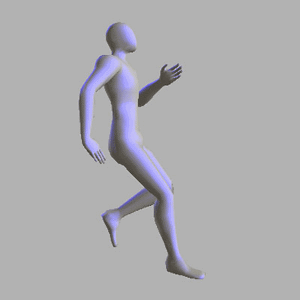
\includegraphics[width=0.5cm]{Icons/inverse_icon.png} on the left side tool bar. Inverse simulation can take up to one hour depending on the number and speed of the CPUs of the computer being used for the simulation. Wait until the deterministic inverse modeling and the MCMC is finished. The progress bars on the \textbf{Simulation} window shows the percentage of each stage on inverse modeling being completed (Figures \ref{fig:43} and \ref{fig:44}). 

\begin{figure}[!ht]
\begin{center}
\includegraphics[width=8cm]{Images/Figure43.png} \\
\caption{Inverse modeling progress window during deterministic parameter estimation stage}\label{fig:43}
\end{center}
\end{figure}  

\begin{figure}[!ht]
\begin{center}
\includegraphics[width=8cm]{Images/Figure44.png} \\
\caption{Inverse modeling progress window during probabilistic parameter estimation}\label{fig:44}
\end{center}
\end{figure}  



\item \textbf{Estimated values of the parameters: } To see the estimated values of the parameters select a parameter from \textbf{Project Explorer}$\rightarrow$\textbf{Inverse Modeling}$\rightarrow$\textbf{Parameters} and look at the \textbf{Value} field. The value should be replaced by the estimated parameter value. 

\item \textbf{Checking the model vs. observed agreement: } Right-click on \textbf{Project Explorer}$\rightarrow$\textbf{Inverse Modeling}$\rightarrow$\textbf{Observations}$\rightarrow$\textit{DO\_nospike} and the choose \textbf{Plot modeled data}. A graph will appear that will show observed data and the model prediction based on the estimated parameters. Do the same for other observation data (Figure \ref{fig:48}).

\begin{figure}[!ht]
\begin{center}
\includegraphics[width=10cm]{Images/Figure48.png} \\
\caption{Observed and predicted DO variation in all four experiments}\label{fig:48}
\end{center}
\end{figure}  



\item \textbf{Checking the posterior distributions of the parameters: }\\ - From \textbf{Project Explorer}$\rightarrow$\textbf{Inverse Modeling}$\rightarrow$\textbf{Parameters} right-click on $\mu_{NOB}$ and select \textbf{Plot posterior distribution histogram}. A graph will appear that shows the posterior distribution of parameter $\mu_{NOB}$ (Figure \ref{fig:45}). Similarly inspect the posterior distribution for other parameters. (Figure \ref{fig:46}). In this figure the box plot shows the 95\% credible interval for the parameter while the solid line shows the median and the dot shows the expected value of the parameter. 

\begin{figure}[!ht]
\begin{center}
\includegraphics[width=11cm]{Images/Figure45.png} \\
\caption{Posterior distribution of $k_{OH}$,  $\mu_{OHO}$, $k_{ON}$,  $\mu_{NOB}$}\label{fig:45}
\end{center}
\end{figure}  


\begin{figure}[!ht]
\begin{center}
\includegraphics[width=8cm]{Images/Figure46.png} \\
\caption{Posterior credible interval for }\label{fig:46}
\end{center}
\end{figure}  


- To see the 95\% credible intervals for all the parameters right-click on \textbf{Project Explorer}$\rightarrow$\textbf{Inverse Modeling}$\rightarrow$\textbf{Parameters} and select \textbf{Plot Percentile data} (Figure \ref{fig:47}). 


-  From \textbf{Project Explorer}$\rightarrow$\textbf{Inverse Modeling}$\rightarrow$\textbf{Parameters} right-click on $\mu_{NOB}$ and select \textbf{Plot percentiles}. 

\begin{figure}[!ht]
\begin{center}
\includegraphics[width=8cm]{Images/Figure47.png} \\
\caption{Posterior credible interval for all parameters}\label{fig:47}
\end{center}
\end{figure} 

\end{itemize}
\section{Maximum-likelihood Inverse Modeling Control Parameters}

This section describes the control parameters for the maximum-likelihood (deterministic) inverse modeling feature of GIFMod. The maximum-likelihood control parameters can be accessed through \textbf{Project Explorer}$\rightarrow$\textbf{Inverse Modeling}$\rightarrow$\textbf{Genetic Algorithm}.

\begin{itemize}
    \item \textbf{Name: } The name of Genetic Algorithm object. It can be ignored. 
    \item \textbf{Cross-over probability: } This indicates the probability of \textit{individuals} undergoing a cross-over to generate the \textit{off-springs}. The reminder of the \textit{individuals} selected for mating will be copied to the next generations with only \textit{mutation}. For example if the value of \item \textbf{Cross-over probability} is set to 0.8, 80\% of the selected individuals will undergo cross-over while 20\% will be directly copied to the next generation. 
    \item \textbf{GA output file: } The results of genetic algorithm optimization will be written in this file. The file that will be generated can be used for diagnosis of the GA performance. 
    \item \textbf{Initial GA population: } If a file name is provided here it will be considered as the initial population for the GA analysis. If this field is empty, the initial GA population will be created randomly. 
    \item{Mutation probability: } This indicates the probability of mutation of each bit when copying from one generation to the other.
    \item{Number of generations: } Indicates the number of generation in the GA algorithm to obtain the optimal parameter set.
    \item{Perform local sensitivity analysis: } Indicates whether a local sensitivity analysis should be performed based on the deterministic parameter obtained by the GA algorithm. The results of the local sensitivity analysis will be saved in a text file called "sensitivity\_mat\_lumped.txt" in the working path. 
    \item{Population: } Indicates the population number that will be used for the GA optimization.
    \item{Read GA analysis from file: } This field is used when the GA analysis has been previously done and only the post-processing is intended to be done using the results of the previous inverse modeling. The file name that will be entered is where GIFMod will load the results of the previous GA analysis from.
    \item{Shake scale: } When the maximum fitness in the population is not improved in three sequential generations, an offspring of the fittest individual is produced by adding a random noise to the parameter values. This scale indicate the magnitude of the random noise. The default value is 0.05 which indicate adding a normally distributed noise with a standard deviation equal to 5\% of the value of each parameter. The purpose of this \textit{shaking} is to find possible optimal solution in the neighborhood of the parameter set represented by the fittest individual. 
    \item{Shake scale reduction factor: } If adding the noise does not result in an improved fitness, the shake-scale is gradually reduced (so a closer neighborhood is searched). The shake scale reduction factor is the factor by which this reduction in the shake scale is done. 
    \item{Number of threads: } The number of CPU threads used for the GA and MCMC parameter estimation. 
\end{itemize}

\section{Probabilistic Inverse Modeling Control Parameters}
This section describes the control parameters for the MCMC (stochastic) inverse modeling feature of GIFMod. The MCMC control parameters can be accessed through \textbf{Project Explorer}$\rightarrow$\textbf{Inverse Modeling}$\rightarrow$\textbf{Markov chain Monte Carlo}.

\begin{itemize}
\item \textbf{Create output realization including observation errors} Switching this property to \textit{Yes} results in GIFMod to generate prediction confidence intervals while considering the observation error. 

\item \textbf{Generate output realizations: } Determines whether output realizations based on parameter samples from the posterior distribution should be generated. These realization will be used to determine confidence intervals of model predictions while accounting for parameter uncertainty. 
\item \textbf{Initial perturbation: } Determines whether the initial MCMC parameter sets should be obtained by perturbing the deterministically estimated parameters using GA or by using the non-perturbed values. MCMC used the parameters estimated by the GA as the initial point wither after perturbing the parameters or not. 
 \item{Save realization outputs in a file: } Switching this property to \textit{Yes}, forces the program to create a file where the sampled parameter values from the posterior distribution to generate the posterior realizations are saved. 
 
 